\chapter{Zbiorniki w kaskadzie}
W celu zapoznania się z dokładnym mechanizmem działania modeli Hammersteina i Wienera z realizacją nieliniowej statyki za pomocą modeli rozmytych typu Takagi - Sugeno wybrano obiekt zbiorników ustawionych w kaskadzie. Szczegółowy opis dynamiki i regulacji obiektów tego typu przedstawili autorzy w [Zbiorniki Bakun]. Dokładnie zilustrowali nieliniową dynamikę - w tym przypadku - trzech zbiorników w kaskadzie. w niniejszej pracy skupiono się na dwóch zbiornikach, jeden w kształcie walca o stałym przekroju poprzecznym, natomiast drugi w kształcie stożka o zmieniającej się powierzchni przekroju wraz z wysokością, co wprowadza dodatkową nieliniowość dynamiki. Obiekt zaprezentowano na Rys. \ref{schemat}, natomiast równania opisujące model fizyczny zapisano poniżej:
\begin{equation}
\begin{cases}
\frac{dV_1}{dt} = F_1 + F_D - F_2(h_1) \\[10pt]
\frac{dV_2}{dt} = F_2(h_1) - F_3(h_2) \\[10pt]
F_2(h_1) = \alpha_1 \sqrt{h_1}, \quad F_3(h_2) = \alpha_2 \sqrt{h_2}, \quad V_1(h_1) = A_1h_1, \quad V_2(h_2) = C_2h_2^2, \quad F_1(t) = F_{1in}(t-\tau)  
\end{cases}
\label{model_fiz}
\end{equation}

\begin{itemize}
\item[•] Stałe: 
\begin{equation}
A_1 = 540\ cm^2, \quad C_2 = \num{0.85}, \quad \alpha_1 = 26, \quad \alpha_2 = 20
\end{equation}

\item[•] Punkt pracy:
\begin{equation}
F_1 = 90\ \frac{cm^3}{s}, \quad F_D = 30\ \frac{cm^3}{s}, \quad \tau = 100\ s, \quad h_2 = 36\ cm
\end{equation}
\end{itemize}

Wartością sterującą był dopływ $F_{1in}$ natomiast zakłóceniem - $F_D$. Z kolei wyjściem - wartością regulowaną - wysokość cieczy w drugim zbiorniku $h_2$. Pozostałe oznaczenia:
\begin{itemize}
\item[•] $A_1$ - stałe pole przekroju poprzecznego pierwszego zbiornika\\
\item[•] $C_2$, $\alpha_1$, $\alpha_2$ - stałe opisujące przepływ cieczy między zbiornikami\\
\item[•] $\tau$ - stała czasowa, opisująca opóźnienie z jakim sterowanie $F_1$ działa na układ\\
\item[•] $h_1$ - wysokość cieczy w pierwszym zbiorniku\\
\end{itemize}

\noindent Użyte oznaczenia odpowiadają tym zastosowanym na rys. \ref{schemat}. 

\newpage

\begin{figure}[h!]
\centering
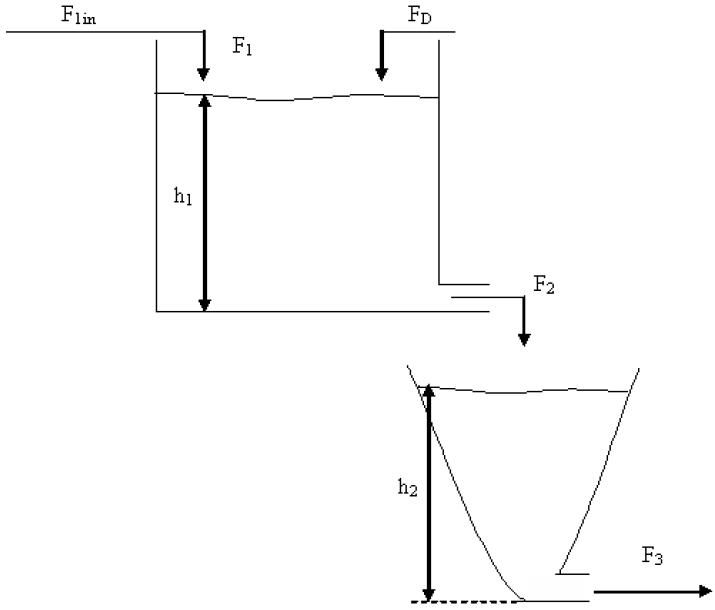
\includegraphics[width=\textwidth]{pictures/schemat}
\caption{Obiekt regulacji automatycznej.}
\label{schemat}
\end{figure}

Plan pracy podzielono na kilka kluczowych aspektów:

\begin{enumerate}
\item Dokonano identyfikacji modelu sprawdzono jego nieliniowość, poprzez wykreślenie charakterystyk statycznych.
\item Zlinearyzowano obiekt w punkcie pracy i wygenerowano wymuszenia skokowe, aby sprawdzić niedokładność modelu liniowego.
\item Dokonano identyfikacji modeli Hammersteina i Wienera. Nieliniową statykę zrealizowano zarówno stosując standardowe podejście - liniowe następniki modeli Takagi - Sugeno - jak i z wykorzystaniem następników hiperbolicznych. 
\item Zaimplementowano regulator DMC w kilku wariantach, porównano działanie regulatorów i wybrano najlepszy.
\end{enumerate}